% \date{May 14, 2024}
% \author{Deralive}
% \title{华东师范大学软件学院实验报告模板}
% 注意事项:编译两次,以确保目录、页码完整显示

\def\allfiles{}

%————————————多文件编译————————————%
% \ifx\allfiles\undefined
% 	    \begin{document}
% \else
% \fi

% Content

% \ifx\allfiles\undefined
% 	    \end{document}
% 	\else
% 	\fi
%—————————————————————————————————%

\documentclass[14pt,a4paper,UTF8,twoside]{article}

\usepackage{amsmath}
\usepackage{graphicx}
\usepackage{geometry} 
\usepackage{ctex}
\usepackage{booktabs} % 表格库
\usepackage{titlesec} % 标题库
\usepackage{fancyhdr} % 页眉页脚库
\usepackage{lastpage} % 页码数库
\usepackage{listings} % 代码块包
\usepackage{xcolor}
\usepackage[hidelinks]{hyperref}
\usepackage{tikz}
\usepackage{tikz-qtree}
\usepackage{fontspec} % 允许设置字体
\usepackage{unicode-math} % 允许数学公式使用特定字体
\usepackage{mwe}
\usepackage{zhlipsum} % 中文乱数文本
\usepackage{amsmath}
\usepackage{xcolor}
\usepackage{float} % 浮动体环境
\usepackage{subcaption} % 子图包
\usepackage{biblatex}
\addbibresource{references.bib} % 指定你的.bib文件名称

\definecolor{mygreen}{rgb}{0,0.6,0}
\definecolor{mygray}{rgb}{0.5,0.5,0.5}
\definecolor{mymauve}{rgb}{0.58,0,0.82}

\date{} % 留空,以让编译时去除日期

%———————————————注意事项—————————————————%

% 1、如果编译显示失败,但没有错误信息,就是 filename.pdf 正在被占用
% 2、在文件夹中的终端使用 Windows > xelatex filename.tex 也可编译

%—————————————华东师范大学———————————————%

% 论文制作时须加页眉,页眉从中文摘要开始至论文末
% 偶数页码内容为:华东师范大学硕士学位论文,奇数页码内容为学位论文题目

%————————定义 \section 的标题样式————————%

% 注意:\chapter 等命令,内部使用的是 \thispagestyle{plain} 的排版格式
% 若需要自己加上页眉,实际是在用 \thispagestyle{fancy} 的排版格式
% 加上下面这一段指令,就能够让 \section 也使用 fancy 的排版格式
% 本质就是让目录、第一页也能够显示页眉、页脚

\fancypagestyle{plain}{
  \pagestyle{fancy}
}

\title{华东师范大学软件学院课程作业} % 模板
\titleformat{\section}
    {\normalfont\bfseries\Large} % 字体大小、字体系列(\bfseries 为加粗)
    {\thesection}{1em}{}

% 设置章节的中文格式
\renewcommand\thesection{\chinese{section} \hspace{0pt}}
\renewcommand\thesubsection{\arabic{subsection} \hspace{0pt}}
% \renewcommand\thesubsubsection{\alph{subsubsection} \hspace{0pt}} % 字母编号
% \hspace{0pt} 是为了确保在章节编号和章节题目之间不要有空格,使得排版更为美观
    
%—————————————页面基础设置———————————————%

\geometry{left=10mm, right=10mm, top=20mm, bottom=20mm}

%————————————设置页眉、页脚——————————————%

\pagestyle{fancy} % 设置 plain style 的属性

% 设置页眉

\fancyhead[RE]{\leftmark} % Right Even 偶数页右侧显示章名 \leftmark 最高级别章名
\fancyhead[LO]{\rightmark} % Left Odd 奇数页左侧显示节名 \rightmark 第二级别节名
\fancyhead[C]{华东师范大学软件学院课程作业} % Center 居中显示
\fancyhead[LE,RO]{~\thepage~} % 在偶数页的左侧,奇数页的右侧显示页码
\renewcommand{\headrulewidth}{1.2pt} % 页眉与正文之间的水平线粗细

% 设置页脚:在每页的右下脚以斜体显示书名

\fancyfoot[RO,RE]{\it Lab Report By \LaTeX} % 使用意大利斜体显示
\renewcommand{\footrulewidth}{0.5pt} % 页脚水平线宽度

% 设置页码:在底部居中显示页码

\pagestyle{fancy}
\fancyfoot[C]{\kaishu 第 \thepage 页 \ 共 \pageref{LastPage} 页} % LastPage 需要二次编译以获取总页数

%——————————————代码块设置———————————————%

\lstset {
    backgroundcolor=\color{white},   % choose the background color; you must add \usepackage{color} or \usepackage{xcolor}
    basicstyle=\footnotesize,        % the size of the fonts that are used for the code
    breakatwhitespace=false,         % sets if automatic breaks should only happen at whitespace
    breaklines=true,                 % sets automatic line breaking
    captionpos=bl,                   % sets the caption-position to bottom
    commentstyle=\color{mygreen},    % comment style
    deletekeywords={...},            % if you want to delete keywords from the given language
    escapeinside={\%*}{*},           % if you want to add LaTeX within your code
    extendedchars=true,              % lets you use non-ASCII characters; for 8-bits encodings only, does not work with UTF-8
    frame=single,                    % adds a frame around the code
    keepspaces=true,                 % keeps spaces in text, useful for keeping indentation of code (possibly needs columns=flexible)
    keywordstyle=\color{blue},       % keyword style
    % language=Python,               % the language of the code
    morekeywords={*,...},            % if you want to add more keywords to the set
    numbers=left,                    % where to put the line-numbers; possible values are (none, left, right)
    numbersep=5pt,                   % how far the line-numbers are from the code
    numberstyle=\tiny\color{mygray}, % the style that is used for the line-numbers
    rulecolor=\color{black},         % if not set, the frame-color may be changed on line-breaks within not-black text (e.g. comments (green here))
    showspaces=false,                % show spaces everywhere adding particular underscores; it overrides 'showstringspaces'
    showstringspaces=false,          % underline spaces within strings only
    showtabs=false,                  % show tabs within strings adding particular underscores
    stepnumber=1,                    % the step between two line-numbers. If it's 1, each line will be numbered
    stringstyle=\color{orange},      % string literal style
    tabsize=2,                       % sets default tabsize to 2 spaces
    % title=Python Code              % show the filename of files included with \lstinputlisting; also try caption instead of title
}

% 注释掉的部分用于后续插入代码,参数可调整,格式如下:

% 1、直接插入
% \begin{lstlisting}[language = ? , title = { ? } ]
%       Your code here.
% \end{lstlisting}

% 2、文件插入
% \lstinputlisting[language = C , title = ?.c] {filename.c}

%———————————————字体设置————————————————%

% \setCJKmainfont{SimSun} % 设置正文罗马族的 CJK 字体
% \renewcommand{\normalsize}{\fontsize{12pt}{15pt}\selectfont} % 设置正文字号
\linespread{1.2}

%——————————————————————————————————————%

%———————————————超链接设置——————————————%

\hypersetup{
    pdfstartview=FitH, % 设置PDF文档打开时的初始视图为页面宽度适应窗口宽度(即页面水平适应)
    CJKbookmarks=true, % 用对CJK(中文、日文、韩文)字符的书签支持,确保这些字符在书签中正确显示
    bookmarksnumbered=true, % 书签带有章节编号。这对有章节编号的文档很有用
    bookmarksopen=true, % 文档打开时,书签树是展开的,方便查看所有书签
    colorlinks, % 启用彩色链接。这样,链接在PDF中会显示为彩色,而不是默认的方框
    pdfborder=001, % 设置PDF文档中链接的边框样式。001 表示链接周围没有边框,仅在单击时显示一个矩形
    linkcolor=blue, % 设置文档内部链接(如目录中的章节链接)的颜色为蓝色
    anchorcolor=blue, % 设置锚点链接(即目标在同一文档内的链接)的颜色为蓝色
    citecolor=blue, % 设置引用(如文献引用)的颜色为蓝色
}

%——————————————导言区结束,进入正文部分———————————————%

%——————————————————————————————————————%

\begin{document}

\maketitle

\begin{center} % \extracolsep{\fill} 拉伸到页面最大宽度前,保证居中显示

  \begin{tabular*}{\textwidth}{@{\extracolsep{\fill}} l  l  l }
    \hline
    课程名称:计算机网络 &  年级:2023级本科  &  姓名:张梓卫 \\
    作业主题:第三章作业 & 学号:10235101526 & 作业日期:2024/11/05 \\
    指导老师:刘献忠 & 组号: \\
    \hline
  \end{tabular*}

\end{center}

% \tableofcontents % 目录也需要二次编译

\section{3.1}

3-1. The following data fragment occurs in the middle of a data stream for which the byte stuffing algorithm described in the text is used: A B ESC C ESC FLAG FLAG D. What is the output after stuffing?

下列数据片段出现在数据流的中间,使用字节填充算法处理后的数据流为:A B ESC C ESC FLAG FLAG D。经过填充后,输出是什么?

\subsection*{解答}

根据题意,遇到ESC或FLAG时需要进行字节填充,将这些特殊字符前面插入一个ESC。例如:

\begin{itemize}
  \item ESC变为ESC ESC
  \item FLAG变为ESC FLAG
\end{itemize}

原数据流为:A B ESC C ESC FLAG FLAG D。

经过字节填充后,数据变为:A B ESC ESC C ESC ESC ESC FLAG ESC FLAG D。

\section{3.2}

3-2. Can you think of any circumstances under which an open-loop protocol (e.g., a Hamming code) might be preferable to the feedback-type protocols discussed throughout this chapter?

你能想到在什么情况下开环协议(例如汉明码)比本章讨论的反馈类型协议更有利吗?

\subsection*{解答}

在以下情况下可能优于反馈协议:

\begin{itemize}
  \item 在发送时间很长时,反馈协议需要确认和应答,增加了往返时间。在低延迟高效率场景中,汉明码更合适。
  \item 信道误码率低,可用汉明码来纠正少数错误,而无需每次都发送确认。
  \item 若需要广播数据,开放式协议可以减少开销,因为接收方不需要回复确认。
\end{itemize}

\section{3.3}

3-3. An 8-bit byte with binary value 10101111 is to be encoded using an even-parity Hamming code. What is the binary value after encoding?

一个8位字节的二进制值是 10101111,要求使用偶校验汉明码进行编码。编码后的二进制值是多少?

\subsection*{解答}

对于汉明码编码,我们需要在数据流中插入校验位,使它们位于 2 的幂次方位置(如第 1 位、第 2 位、第 4 位、第 8 位等)。这些校验位用于检查特定位置的比特是否满足偶校验。

初始结构如下所示:

\begin{lstlisting}[language=C]
  p1 p2 1 p4 0 1 0 p8 1 1 1 1
\end{lstlisting}

需要校验的位判断方法如下:

\textbf{按二进制掩码确定}

\begin{itemize}
  \item p1(1 = 0001)校验所有二进制表示的最后一位为 1 的位置(如 1, 3, 5, 7, 9, 11...)。
  \item p2(2 = 0010)校验所有二进制表示的倒数第二位为 1 的位置(如 2, 3, 6, 7, 10, 11...)。
\end{itemize}

当检查出有奇数个时,$p_{i}$ 要设置为 1,否则为 0,依次来满足或保持偶校验。

最终结果如下所示:
\begin{lstlisting}
  1 0 1 0 0 1 0 0 1 1 1 1
\end{lstlisting}

\section{3.4}

3-4. What is the remainder obtained by dividing $x^7 + x^5 + 1$ by the generator polynomial $x^3 + 1$?

求余数:$\frac{x^7 + x^5 + 1}{x^3 + 1}$。

\subsection*{解答}

\begin{figure}[H]
  \centering
  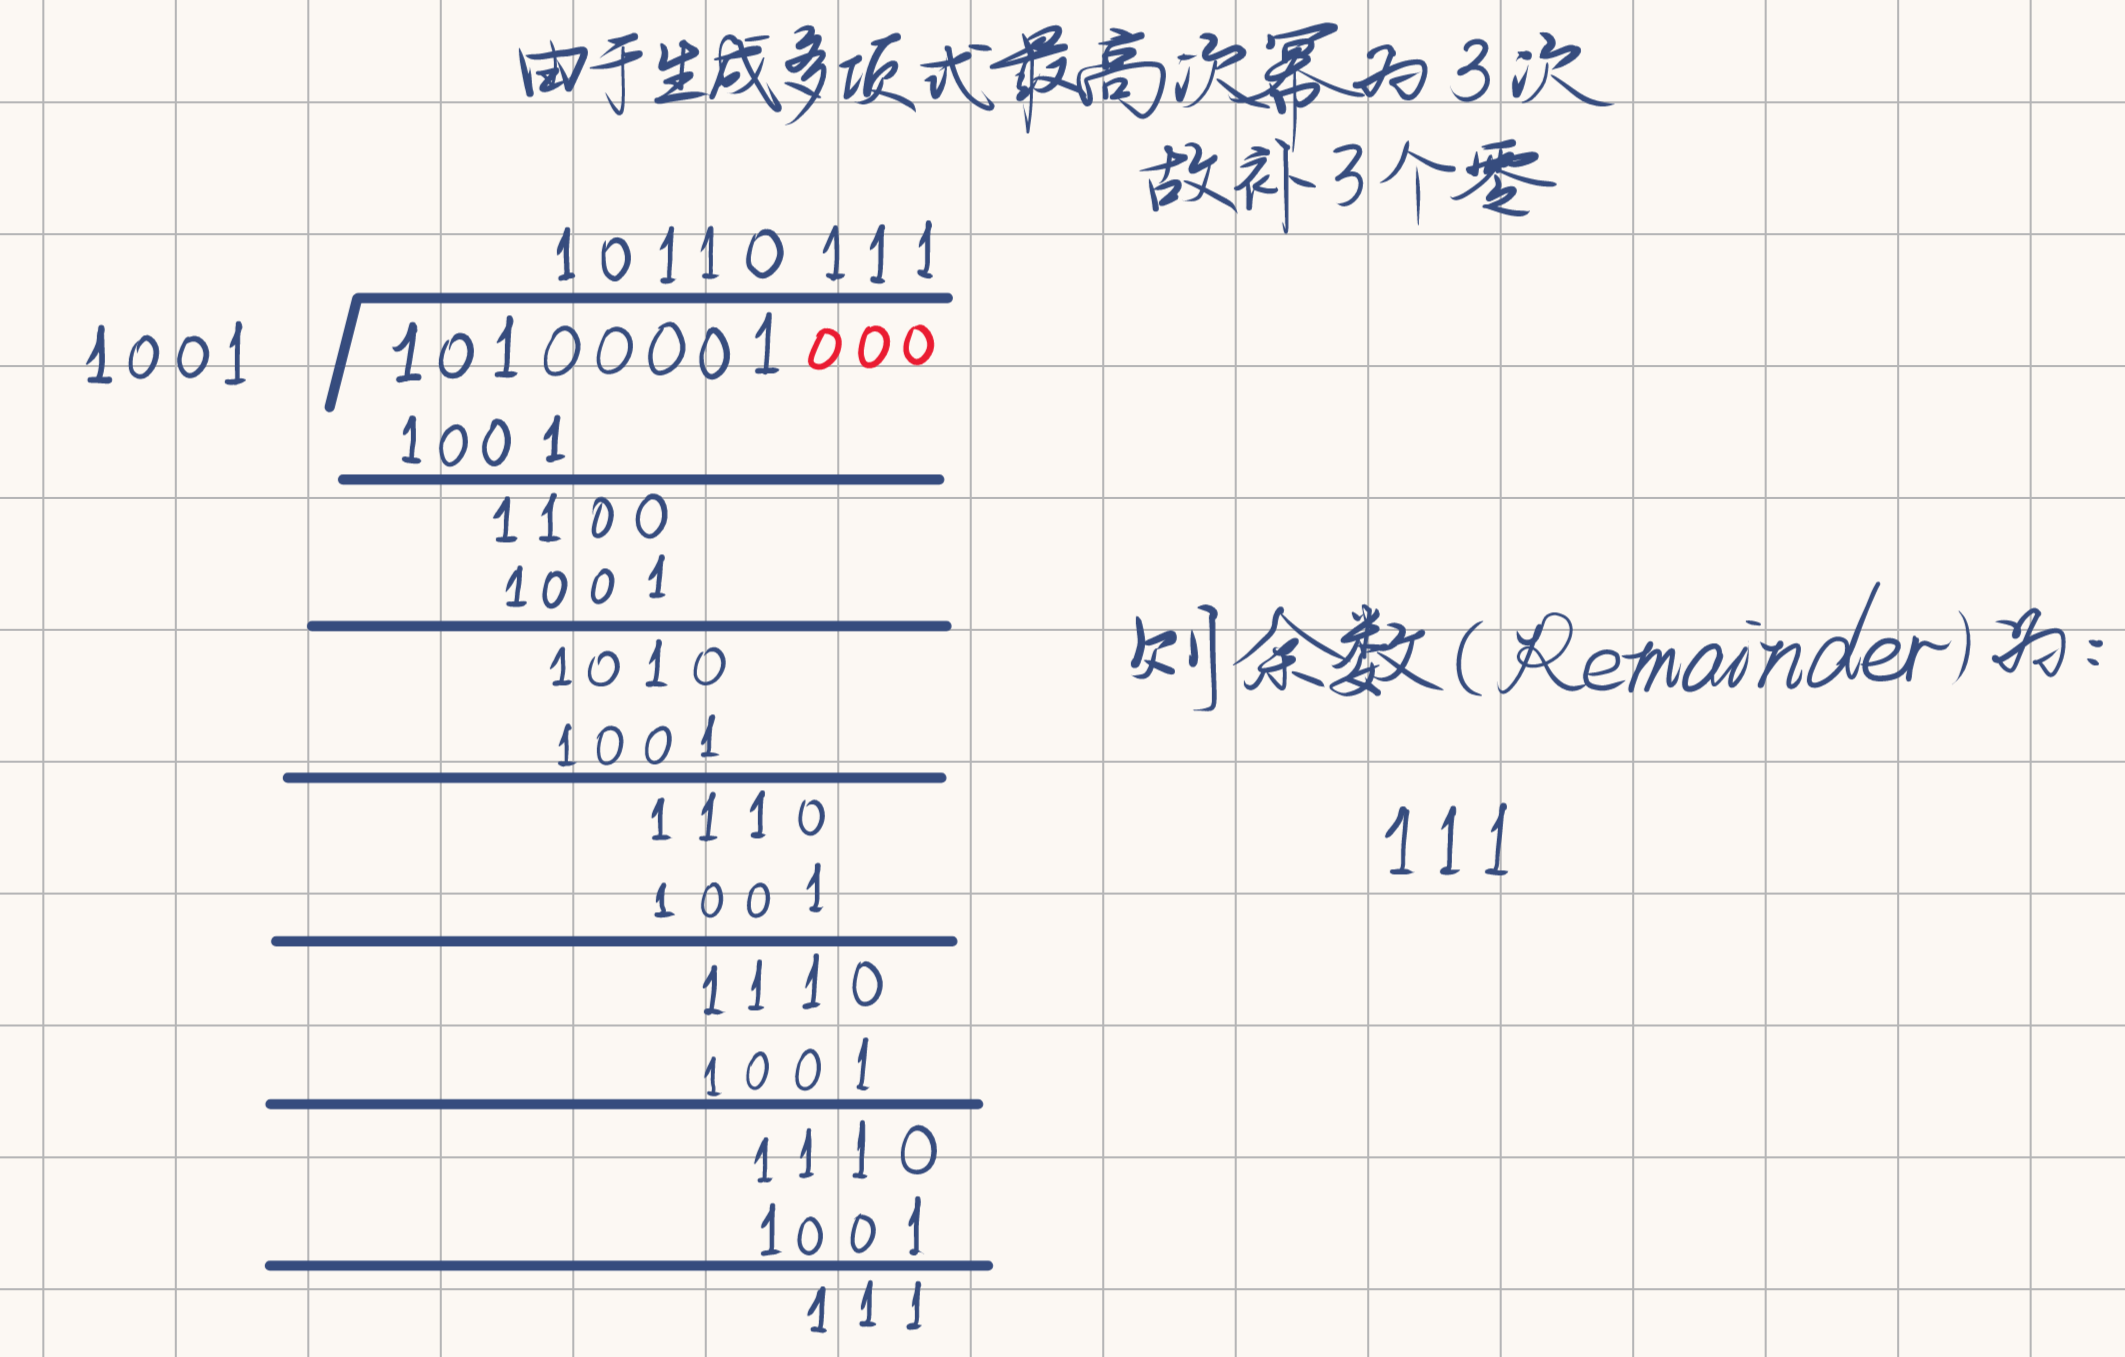
\includegraphics[width=0.5\textwidth]{lec3/Hamming.png}
  \caption{Hamming code}
\end{figure}

故最后答案为 111.

\section{3.5}

3-5. Suppose that a message 1001 1100 1010 0011 is transmitted using Internet Checksum (4-bit word). What is the value of the checksum?

假设消息 1001 1100 1010 0011 采用互联网校验和(4位字)进行传输。校验和的值是多少?

\subsection*{解答}

进行二进制加法,若有进位则加回到第一位:

(1001 + 1100 + 1010 + 0011) = 100010

进位被加到最低有效位,得到 0100.
最后求反码即可。

Checksum = (0100)' = 1011.

\section{3.6}

3-6. A channel has a bit rate of 4 kbps and a propagation delay of 20 msec. For what range of frame sizes does stop-and-wait give an efficiency of at least 50%?

某通道的比特率为4 kbps,传播延迟为20毫秒。对于多大范围的帧大小,停等协议能够达到至少50\%的效率?

\subsection*{解答}

Stop-and-Wait 协议的效率计算公式:

\[
\text{效率} = \frac{\text{帧传输时间}}{\text{帧传输时间} + 2 \times \text{传播延迟}}
\]

已知条件:

\begin{itemize}
  \item 比特率 \( R = 4 \text{ kbps} = 4000 \text{ bps} \)
  \item 传播延迟 \( T_p = 20 \text{ msec} = 0.020 \text{ 秒} \)
  \item 帧大小 \( F \)(以比特为单位)
\end{itemize}

\[
\text{帧传输时间} = \frac{F}{R}
\]

代入求解 $\text{效率} > 50\% $ 的不等式:

\[
\frac{F}{4000} \geq 2 \times 0.020
\]

\[
F \geq 160 \text{ 比特}
\]

故为了使停等协议的效率至少为 50\%,帧大小 \( F \) 必须满足 $ F \geq 160 \text{比特} $

\section{3.7}

3-7. A 3000-km-long T1 trunk is used to transmit 64-byte frames using protocol 5. If the propagation speed is 6 μsec/km, how many bits should the sequence numbers be?

一条3000公里长的T1干线用于使用协议5传输64字节帧。如果传播速度是6 μs/km,序列号应该是多少位?

\subsection*{解答}

   \[
   \text{传播延迟} = 3000 \, \text{km} \times 6 \, \mu\text{s/km} = 18000 \, \mu\text{s} = 18 \, \text{ms}
   \]

   帧大小为 64 字节,即 \(64 \times 8 = 512\) 位。

   使用 T1 线路的传输速率为 1.544 Mbps,即 1.544 Mbits/s 或 1544 bits/ms。

   \[
   \text{帧传输时间} = \frac{512 \, \text{bits}}{1544 \, \text{bits/ms}} \approx 0.33 \, \text{ms}
   \]

   每帧的总时间为传输时间加上传播延迟,再加上回执时间:

   \[
   \text{总时间} = 0.33 \, \text{ms} + 18 \, \text{ms} + 18 \, \text{ms} = 36.33 \, \text{ms}
   \]

   在此时间内信道可以发送的帧数为:

   \[
   \frac{\text{总时间}}{\text{帧传输时间}} = \frac{36.33 \, \text{ms}}{0.33 \, \text{ms}} \approx 121 \text{ 帧}
   \]

   序列号的位数 \( n \) 应满足 \( 2^n \geq 121 \),即

   \[
   2^n \geq 121
   \]

   取 \( n = 7 \) 位即可满足此要求。

\section{3.8}

3-8. In protocol 6, when a data frame arrives, a check is made to see if the sequence number differs from the one expected and no nak is true. If both conditions hold, aNAK is sent. Otherwise, the auxiliary timer is started. Suppose that the else clause were omitted. Would this change affect the protocol’s correctness?

在协议6中,当接收到数据帧时,检查序列号是否与预期值不同且未收到nak。如果这两个条件成立,则发送aNAK。否则,启动辅助计时器。假设省略了else子句。这样做会影响协议的正确性吗?

\subsection*{解答}

Protocol 6 here refers to the Selective Repeat Protocol.

May lead to deadlock. Assuming a set of frames arrives correctly and is received. Then, the receiving end will move the window forward.
But if all the confirmation frames are lost, the sender will timeout and send the first frame again, while the receiver will send a NAK. Then NONAK was set to false.
And it is impossible to know that the frames that have been sent have been received and there is no time limit,
If NAK is also lost, the sender will continue to send frames that have already been accepted by the receiver.
The receiver simply ignores these frames, but since NONAK is fake, it will not send NAK again, resulting in a deadlock.
If an auxiliary counter is set (implementing the 'else' clause) and NAK is resent after timeout, both parties will eventually regain synchronization.

可能导致死锁。假定有一组帧正确到达,并被接收。然后,接收端会向前移动窗口。 
但若确认帧都丢失了,发送端就会超时,会再发送第一帧,接收端将发送一个NAK。然后NONAK 被置成伪。
而无法得知已经发送的帧已被接收,并且没有时间限制,
若 NAK 也丢失,那么发送方会不断发送已经被接收方接受了的帧。
接收方只是忽略这些帧,但由于NONAK 为伪,所以不会再发送NAK,从而产生死锁。
如果设置辅助计数器(实现“else”子句),超时后重发NAK,终究会使双方重新获得同步。

\section{3.9}

3-9. Suppose that the three-statement while loop near the end of protocol 6 was removed from the code. Would this affect the correctness of the protocol or just the performance? Explain your answer.

假设在协议6末尾的三语句while循环被移除。这样会影响协议的正确性还是仅影响性能?请解释你的答案。

\subsection*{解答}

协议6中的三个语句while循环负责检查当前进程的值是否为所有其他进程值中的最小值。它通过将其值发送给所有其他进程并接收它们的值来实现这一点。

移除协议 6 末尾的三语句 while 循环可能会影响协议的正确性。该循环用于确保接收端能够处理并确认所有帧。如果移除它,接收端可能会遗漏某些帧的确认,从而导致发送端重传不必要的帧或造成数据丢失。


\section{3.10}

3-10. Frames of 1000 bits are sent over a 1-Mbps channel using a geostationary satellite whose propagation time from the earth is 270 msec. Acknowledgements are always piggybacked onto data frames. The headers are very short. Three-bit sequence numbers are used. What is the maximum achievable channel utilization for

通过1 Mbps的通道发送1000位的帧,使用地球同步卫星进行传输,地球到卫星的传播时间为270毫秒。确认总是附带在数据帧上。帧头非常短。使用三位序列号。以下协议的最大可实现通道利用率是多少?

\begin{itemize}
  \item (a) 停等协议?
  \item (b) 协议5?
  \item (c) 协议6?
\end{itemize}
\subsection*{解答}

帧的传输时间:
   \[
   T_{\text{frame}} = \frac{\text{帧大小}}{\text{通道容量}} = \frac{1000 \text{ 位}}{1,000,000 \text{ bps}} = 1 \text{ ms}
   \]

由于单程传播延迟为 270 ms,因此往返时间为:
   \[
   RTT = 2 \times 270 \text{ ms} = 540 \text{ ms}
   \]

(a) 停等协议

在停等协议中,发送方发送一个帧后需要等待确认后才能发送下一帧。这意味着在每帧发送之后的往返延迟期间信道都是空闲的。

利用率为:

\[
U = \frac{\text{传输时间}}{\text{传输时间} + \text{往返时间}}
\]
\[
U = \frac{1 \text{ ms}}{1 \text{ ms} + 540 \text{ ms}} = \frac{1}{541} \approx 0.00185
\]

(b) 协议5(回退N协议)

在回退N协议中,窗口大小为 $W=7$(因为我们有三位序列号),发送方可以在等待确认之前最多发送 7 个帧。

回退N的信道利用率可以近似为:
\[
U = \frac{\min(W, \frac{\text{RTT}}{T_{\text{frame}}}) \times T_{\text{frame}}}{\text{RTT} + T_{\text{frame}}}
\]
因为 $ \frac{\text{RTT}}{T_{\text{frame}}} = \frac{540}{1} = 540 $,远大于 $ W = 7 $,我们使用 $ W = 7 $ 进行计算:

\[
U = \frac{7 \times 1 \text{ ms}}{540 \text{ ms} + 1 \text{ ms}} = \frac{7}{541} \approx 0.01294
\]

(c) 协议6(选择重传协议)

在选择重传协议中,每个帧的确认是独立发送的,并且只有出错的帧才会被重传。假设无错误情况下,发送方可以连续发送 7 个帧,并为每个帧接收确认。

由于信道可以在窗口大小范围内连续利用,在无错误条件下,利用率与回退N协议相同。因此:

\[
U = \frac{7 \times 1 \text{ ms}}{540 \text{ ms} + 1 \text{ ms}} = \frac{7}{541} \approx 0.01294
\]

综上所述,答案结果如下:

1. 停等协议: 0.185\%
2. 回退N协议(协议5): 1.294\%
3. 选择重传协议(协议6): 1.294\%

因此,最高可实现的信道利用率在无错误条件下约为 1.294\%,适用于回退N和选择重传协议,假设最大窗口大小为7。


\end{document}